\chapter{Basic Examples}
\label{ch:ch1}

\section{AMS Theorem Styles}

\begin{remark}
	This statement is true, I guess.
\end{remark}

\begin{theorem}
	Let \(f\) be a function whose derivative exists in every point, then \(f\) is a continuous function.
\end{theorem}

\begin{definition}
	The \textbf{centre} of a graph \(G\) is the set of all vertices of minimum eccentricity.
\end{definition}

Let \(V = \{v_1, v_2, \dotsc, v_n\}\) and \(\mathfrak{E} = \{\mathfrak{e}_1, \mathfrak{e}_2, \dotsc, \mathfrak{e}_m\}\). The \(n \times m\) incidence matrix of a hypergraph \(H = (V, \mathfrak{E})\) is a \((0, 1)\)-matrix \(A = (a_{ij})\) where
\begin{equation*}
	a_{i, j} =
	\begin{cases}
		1, & \text{if \(v_i \in \mathfrak{e}_j\)} \\
		0, & \text{otherwise.}
	\end{cases}
\end{equation*}
And easily we\footnote{The word ``we'' refers to two male pandas.} can see that the incidence matrix of \(H\) is just the biajacency matrix of the original graph \cite[pp.~22]{tanenbaum2011computer}.

\section{Tables, Figures and Images}

\lipsum[1]

\begin{table}[ht]
	\centering
	\begin{tabular}{||c c c c||}
		\hline
		Col1 & Col2 & Col2 & Col3 \\ [0.5ex]
		\hline\hline
		1 & 6 & 87837\tablefootnote{This is a footnote in the table.} & 787 \\
		2 & 7 & 78 & 5415 \\
		3 & 545 & 778 & 7507 \\
		4 & 545 & 18744 & 7560 \\
		5 & 88 & 788 & 6344 \\ [1ex]
		\hline
	\end{tabular}
	\caption{Table to test captions and labels}
\end{table}

\lipsum[2]

\begin{figure}[ht]
	\centering
	\includegraphics[width = \textwidth]{Figures/Panda_Cub}
	\caption{A newborn panda cub}
\end{figure}

\lipsum[3]

\begin{figure}[ht]
	\centering
	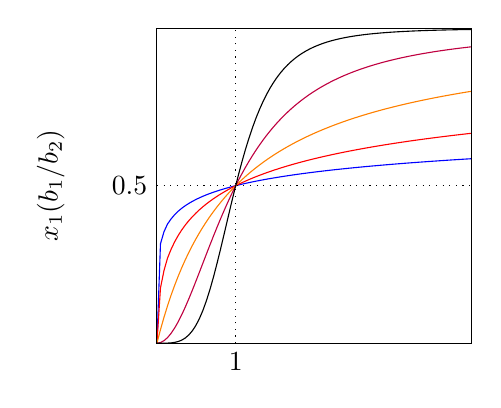
\begin{tikzpicture}[scale = 1]
	\foreach \a/\Col in {0.25/blue, 0.5/red, 1/orange, 2/purple, 4/black}
	{
		\draw[\Col] plot[domain = 0:4, variable = \x, samples = 90] ({\x}, {4 * (\a * \x^\a) / (\a + \a * \x^\a)});
	}
	\draw (0, 0) rectangle (4, 4);
	\draw [dotted] (1, 0) node[below]{$1$} -- (1, 4);
	\draw [dotted] (0, 2) node[left](p5){$0.5$} -- (4, 2);
	\node [left of= p5,rotate = 90]{$x_1(b_1/b_2)$};
\end{tikzpicture}

	\caption{Curves}
\end{figure}

\lipsum[4-5]
